\chapter{Anforderungen an den Prototyp}
\label{cha:Prototyp}

Für den Vergleich der beiden Plugin APIs soll 
in VS Code und in IntelliJ ein möglichst funktionsgleicher 
Prototyp implementiert werden.

Durch diese Prototypen können die Features der beiden APIs 
demonstriert und bewertet werden. Weiters bietet die Entwicklung
der beiden Prototypen
eine praxisnahe Methode, um sich auch mit dem Arbeitsablauf der
beiden Plattformen, speziell auch dem Veröffentlichen
der Plugins, vertraut zu machen.

\section{Aufbau}
\label{sec:Prototyp_Aufbau}

Um diese Aufgaben möglichst gut zu erfüllen, wurde das sogenannte
\enquote{RecentChangesPlugin} entworfen. Es handelt sich 
dabei um ein Plugin, welches Text- oder Codeänderungen 
im Editor mitliest und sich merkt. Dadurch wird die spätere
Wiederholung von gleichen oder ähnlichen Änderungen erleichtert.
Als Änderung wird hierbei das einfache Abändern oder das Ersetzen eines
Wortes durch ein anderes verstanden. 
Das Mitschreiben von komplexeren Veränderungen, zum Beispiel, 
wenn in mehreren Zeilen gleichzeitig Änderungen vorgenommen 
werden, ist nicht Ziel des Prototyps.

\subsection{Beispiel}

Zur besseren Demonstration der Funktionalität wurde folgendes 
Beispiel konstruiert, welches in Abbildung \ref{fig:example_vscode_change-step}
und in Abbildung Abbildung \ref{fig:example_vscode_reapply-step}
zu sehen ist:

Eine Person entwickelt gerade ein Programm und erstellt 
in der Datei \emph{Main.java} einige statische Variablen.
Nun bemerkt die Person, dass es sich bei den Variablen 
\emph{someValue2} und \emph{someValue4} eigentlich um 
Werte vom Typ \emph{double} handelt. Sie macht daher eine 
erste Änderung und passt den Datentyp von \emph{someValue2} an.
Wie in Abbildung \ref{fig:example_vscode_change-step} zu erkennen ist,
bemerkt das Plugin die Änderung und schreibt diese sofort mit.

\begin{figure}
    \centering
    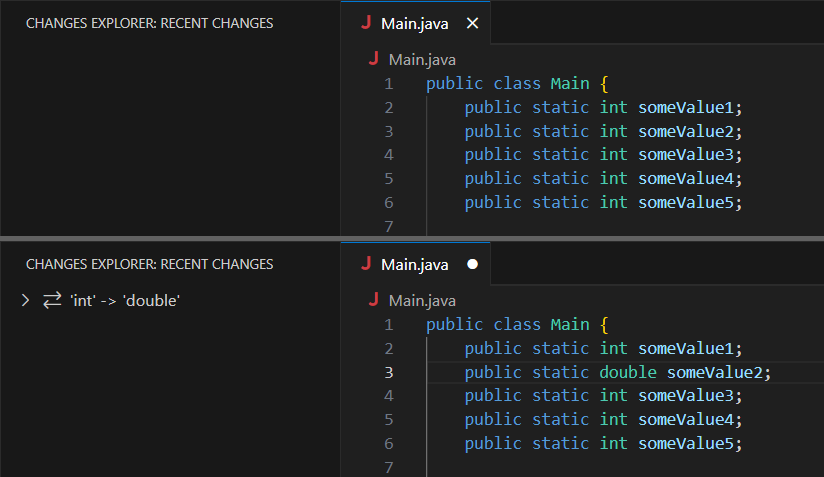
\includegraphics[width=.95\textwidth]{example_vscode_change-step}
    \caption{Mitschreiben einer Änderung durch das \emph{RecentChangesPlugin}.}
    \label{fig:example_vscode_change-step}
\end{figure}

Die Person möchte nun dieselbe Änderung auch noch einmal für
die Variable \emph{someValue4} wiederholen. Sie stellt sich daher
mit dem Cursor an die Position im Text, an der das \emph{int} steht.
Durch das Drücken einer Tastenkombination wird nun die zuvor erkannte
Änderung wieder angewandt und das \emph{int} an der aktuellen Position
wird durch ein \emph{double} ersetzt. Dieser Schritt
ist in Abbildung \ref{fig:example_vscode_reapply-step} zu sehen.

\begin{figure}
    \centering
    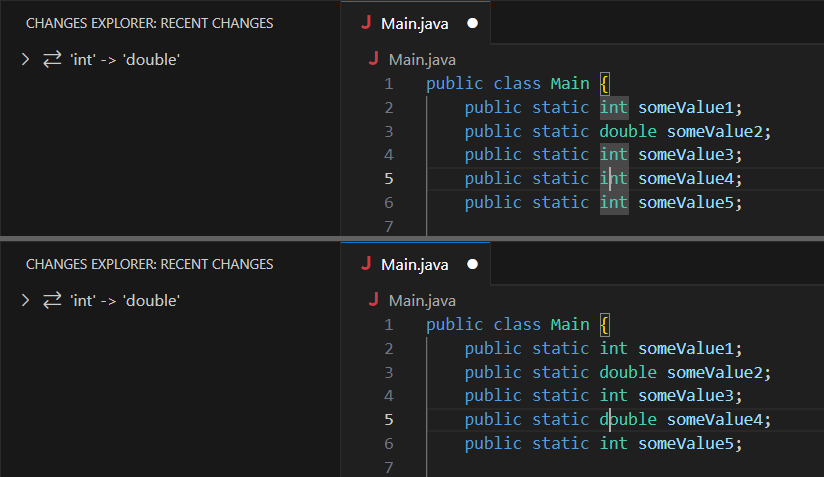
\includegraphics[width=.95\textwidth]{example_vscode_reapply-step}
    \caption{Erneutes Anwenden einer Änderung durch das \emph{RecentChangesPlugin}.}
    \label{fig:example_vscode_reapply-step}
\end{figure}

\subsection{Funktionen}

Für das Plugin wurden folgende Funktionen vorgesehen:

\begin{description}
    \item[Bemerken von Textänderungen] 
    Der Prototyp soll Änderungen in Text- oder Codedateien automatisch
    erkennen, um sich diese zu merken. Um solche Änderungen
    zu erkennen, muss auch erkannt werden, wann eine Änderung 
    vollständig abgeschlossen ist. Hierfür
    soll ein Debounce-Effekt genutzt werden. 
    Dabei wird nach jedem Tastendruck eine gewisse Zeit abgewartet,
    ob noch ein weiterer Tastendruck passiert. Erst wenn
    diese kurze Zeit ohne weitere Tastatureingaben verstreicht, gilt
    die Änderung als abgeschlossen.
    Die erkannten Änderungen müssen analysiert 
    und zwischengespeichert werden.

    \item[Anwenden von Änderungen auf Befehl] 
    Der Prototyp soll zuvor erkannte Änderungen auf Befehl an der
    aktuellen Position im Editor anwenden können. Dafür muss zuerst die
    aktuelle Textcursor-Position analysiert werden, um das Wort zu finden,
    an dem sich der Textcursor befindet. Danach muss in den 
    zwischengespeicherten Änderungen ein passender Eintrag gefunden werden,
    der auch auf die aktuelle Position angewendet werden kann.
    Dabei sollen neuere Änderungen gegenüber älteren bevorzugt werden.

    \item[Anwenden von Änderungen durch Tastenkombination]
    Der Vorgang des An-\linebreak
    wenden von Änderungen soll auch durch eine
    Tastenkombination auslösbar sein.

    \item[Vergessen von alten Änderungen]
    Um erkannte Änderungen nicht ewig im Zwischenspeicher zu halten,
    soll nur eine bestimmte Menge gleichzeitig gespeichert werden 
    können. Wird diese Menge überschritten, so soll die älteste Änderung
    aus dem Zwischenspeicher entfernt und somit \enquote{vergessen} werden.

    \item[Automatische Codevervollständigung]
    Anhand der kürzlichen Änderungen sollen auch Vorschläge
    in der Codevervollständigung angezeigt werden. 
    Da eine Änderung ja immer aus einem entfernten Wort 
    und einem ersetzenden Wort besteht, liegt es hier nahe,
    für die Codevervollständigung nur die ersetzenden Worte
    vorzuschlagen. Die entfernten Worte werden also ignoriert.

    \item[Anzeige der Änderungen]
    Damit die NutzerInnen einen Überblick über die kürzlichen Änderungen
    haben, sollen alle Änderungen, die sich im Zwischenspeicher befinden,
    über eine View angezeigt werden können.

    \item[Einstellungen]
    Es soll möglich sein, Einstellungen des Plugins festzulegen, welche
    auch beim Schließen der Entwicklungsumgebunge persistent bleiben.

    Es soll gespeichert werden:
    \begin{itemize}
        \item wie viele Änderungen gleichzeitig im 
            Zwischenspeicher gehalten werden und
        \item welche Debounce-Zeit für das Erkennen 
            von Änderungen verwendet wird. 
    \end{itemize}

    \item[Tests]
    Es soll eine kleine, demonstrative Menge von Unit- und Integrationstests für
    den Plugin Code geschrieben werden.

\end{description}

% //TODO FIX manual \linebreak